\documentclass[main.tex]{subfiles}
\begin{document}

Discoveries in astronomy have always been directly related to technological advances of new instruments and observation techniques. The first telescope was invented by Galileo in \textit{XVII} century and it allowed him to observe for the first time the four brightest moons of Jupiter. Since then, and specially during the \textit{XX} century, a broad new range of experiments, detectors and telescopes have been built either on the ground or in space. Thanks to them, astronomers have observed the universe in every wavelength from radio to $\gamma$-rays. Furthermore, recently the field of multimessenger astronomy has started a new era, combining light with other cosmic messengers such as neutrinos and gravitational waves.\\

This chapter is dedicated to the technologies used to detect $\gamma$-rays, from the history of first detectors, to the present generation and future of $\gamma$-ray observatories.\\
Contrary to the visible light that Galileo received with his first telescope, $\gamma$-rays cannot be directly observed from Earth. The atmosphere absorbs most of the radiation coming from space, limiting the range of the spectrum that can be detected with ground based detectors. As shown in figure \ref{fig:atmoabsorb}, only visible and radio wavelengths reach the ground through the so called \textit{atmospheric windows}, hence$\gamma$-rays can be observed only from outside the atmosphere, with detectors in balloons or satellites. A description of different types of such detectors and their used techniques is given in section \ref{sec:spacedet}.\\

Other possibility is to take advantage of the interactions of $\gamma$-rays with particles in the atmosphere when they are absorbed. When a $\gamma$-ray or any cosmic particle hits an atmospheric atom, a large number of secondary particles is produced which themselves suffer further interactions in a cascade reaction known as \gls{eas}.
More on \gls{eas} and ground-based detectors can be found in sections \ref{sec:eas} and \ref{sec:grounddet} respectively.\\

Space detectors and ground based detectors complement perfectly well, supplying the limitations of one another to cover the full $\gamma$-ray spectrum. Lower energy $\gamma$-rays are abundant, but so are hadronic backgrounds (\glspl{cr}). Space detectors are perfectly suited to study these part of the spectrum, because beside their rather small collection areas ($\sim 1 m^2$), they have very good background rejection. At higher energies, the $\gamma$-ray flux decay strongly and much higher collection areas are needed to have competitive detectors. Ground based instruments detect the extended secondary products of $\gamma$-rays interacting in the atmosphere, they are designed to cover big areas, capturing even events from the highest energy $\gamma$-rays.\\

\begin{figure}
\centering
 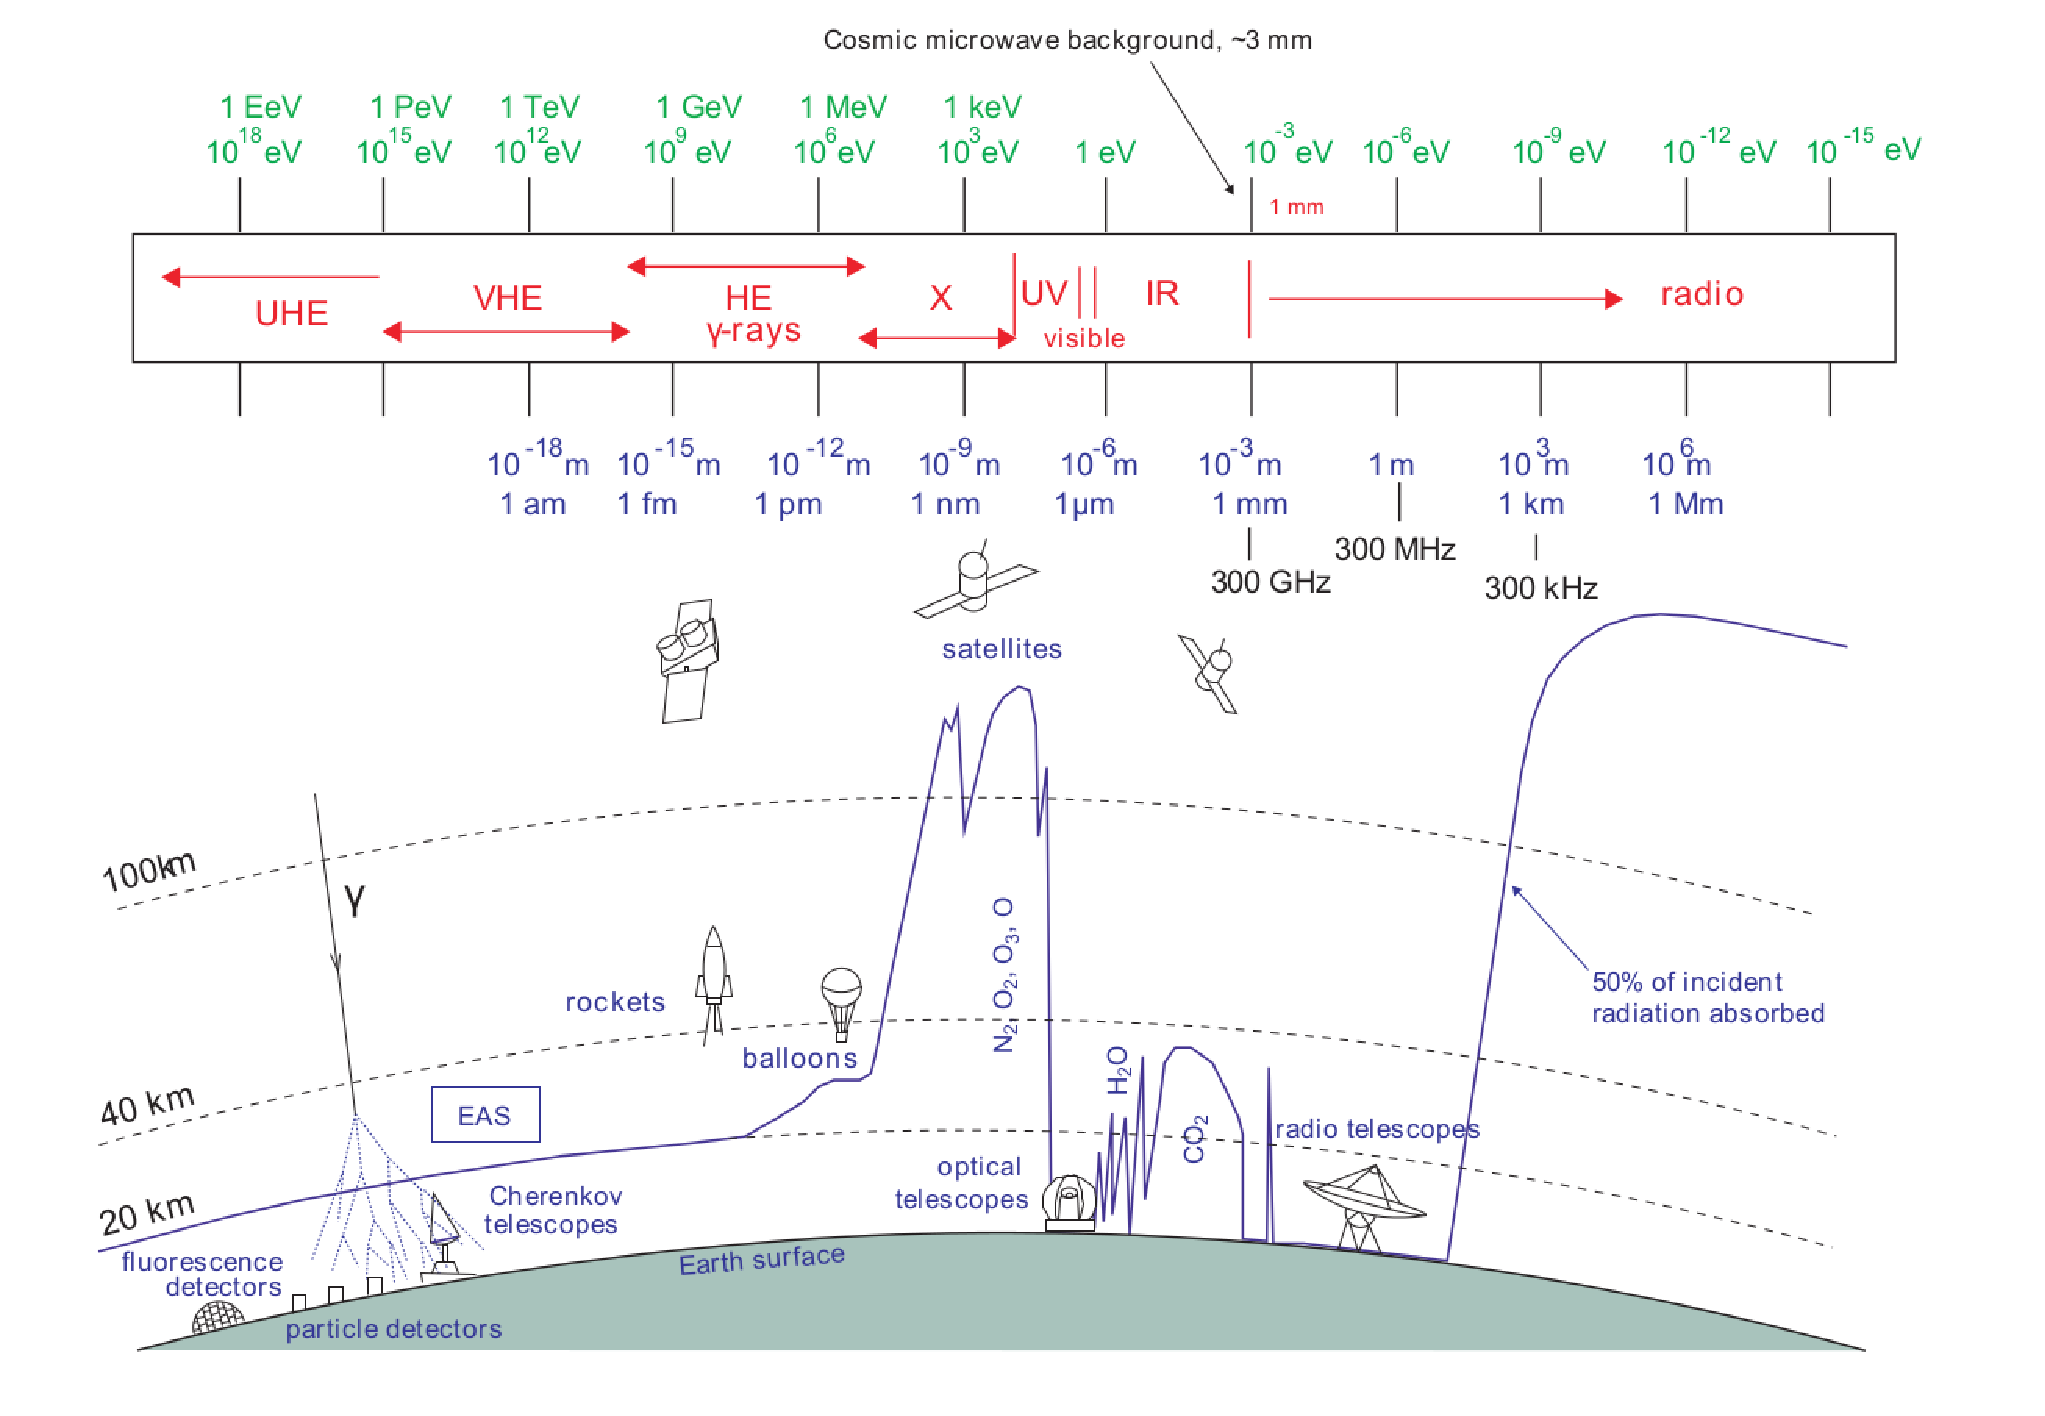
\includegraphics[width=1\textwidth]{EM.pdf}
  \caption{Atmospheric transparency for the whole electromagnetic spectrum, from \cite{highenergyastrophy}. The continuous line represents the height in the atmosphere where 50\% of the light is absorbed.}
    \label{fig:atmoabsorb}
\end{figure}


\section{Space detectors} \label{sec:spacedet}

Direct detection of $\gamma$-rays can only be done outside the atmosphere, with particle detectors mounted in high altitude balloons or satellites. The main advantage of these kind of detectors is the extremely efficient background rejection, being relatively easy to veto charged cosmic particles and distinguish them from neutral $\gamma$ photons. However, they are limited in the energy of the $\gamma$-rays they can observe, not being able to go much further 100 GeV (\gls{he} regime) because of the inability to have a large collection area. The collection area corresponds to the size of the detector, which for space instruments it is about 1 $m^2$, making it very difficult to capture \gls{vhe} photons which flux decreases rapidly with energy.\\
In this section, different types of space detectors are desribed.\\

\subsection{Compton detectors}\label{sec:comptondetectors}

Compton scattering occurs when a photon transfers part of its energy to an electron. At the low end of the $\gamma$-ray energy range (from 20 keV to 30 GeV) this is the process that dominates interactions between light and matter. Compton detectors are based on this interaction. Usually, they count on two parts: In the first level, the interaction between the $\gamma$ photon and an electron occurs inside a scintillator. The trajectory deviation of the photon is measured, and then is possible to reconstruct its original direction. Afterwards, the photon travels to a second level where it is absorbed by a calorimeter and its energy is measured. The \gls{comptel} instrument from the \gls{cgro} was operative between 1991 and 2000 and was able to do a survey of the galactic plane using this technique, detecting more than 60 sources (figure \ref{fig:comptel}). Currently, the \gls{ibis} telescope on board of the \gls{integral} space telescope is the present representative of this kind of detectors.

\begin{figure}
\centering
 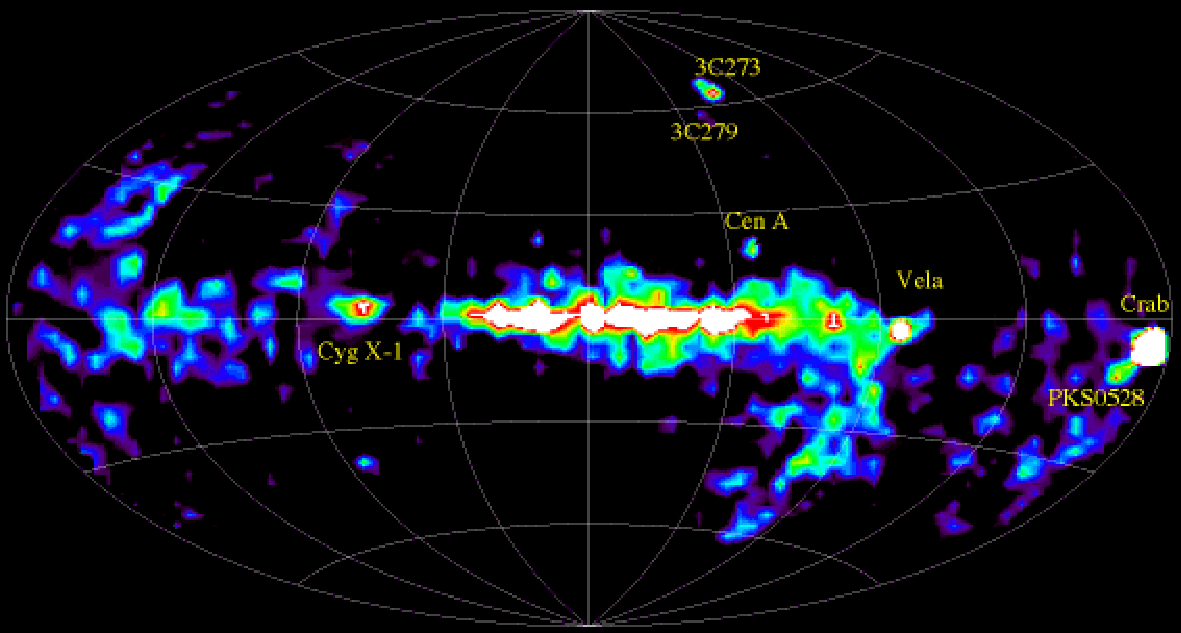
\includegraphics[width=1\textwidth]{Pictures/comptel.pdf}
  \caption{Skymap from \gls{comptel} source catalog. Credits to NASA.}
    \label{fig:comptel}
\end{figure}

\subsection{Pair production detectors} \label{sec:pairprod}

A photon travelling with an energy over twice the rest mass of the electron (511 keV, usually photons over 20 GeV) passing close to a nucleus have a high probability to suffer pair production, meaning it produces an electron-positron pair with kinetic energy.
Pair production detectors account for different layers of a heavy material where the interaction takes place,  interleaved with a tracker material which measures the position of the resulting particles, being able to reconstruct the original direction of the $\gamma$-ray. A calorimeter measures the energy of the particles and an anti-coincidence detector acts as veto for the background of charged particles (\glspl{cr}) which can enter the detector. The latest and most prolific instrument of this kind is the \gls{lat} instrument, on the Fermi Gamma-Ray Telescope which is formerly described in the next section.

\subsubsection{The Fermi Gamma-ray Space Telescope} \label{sec:fermi}

The Fermi Gamma-ray Space Telescope was launched in 2008 with the objective of performing a sky survey in the \gls{he} range. It is placed in a low Earth orbit, being able to observe the whole sky in 3 hours. It accounts of two instruments: The \gls{lat}, which is the principal instrument for $\gamma$-ray detection, and the \gls{gbm}, which is designed to detect \glspl{grb}.\\


\begin{itemize}
    \item \textbf{The \gls{lat}}: This is the principal instrument of the Fermi telescope, a pair production $\gamma$-ray detector able to observe photons with energies between 20 MeV to more than 300 GeV \cite{2009FermiLAT}. It consists on 16 modular towers with 18 tungsten converter layers, where the pair production takes place, and 16 dual silicon tracker planes which measures the position of the $e^{\pm}$ pair. The 16 calorimeter modules have 96 long, narrow CsI scintillators which measure the deposited energy. When any particle enter the detector, they first pass through an anticoincidence plastic scintillator where, if it is a charged particle, it will produce a flash of light, making it possible to distinguish background events from true $\gamma$-ray events.\\
    
    \begin{figure}
    \centering
    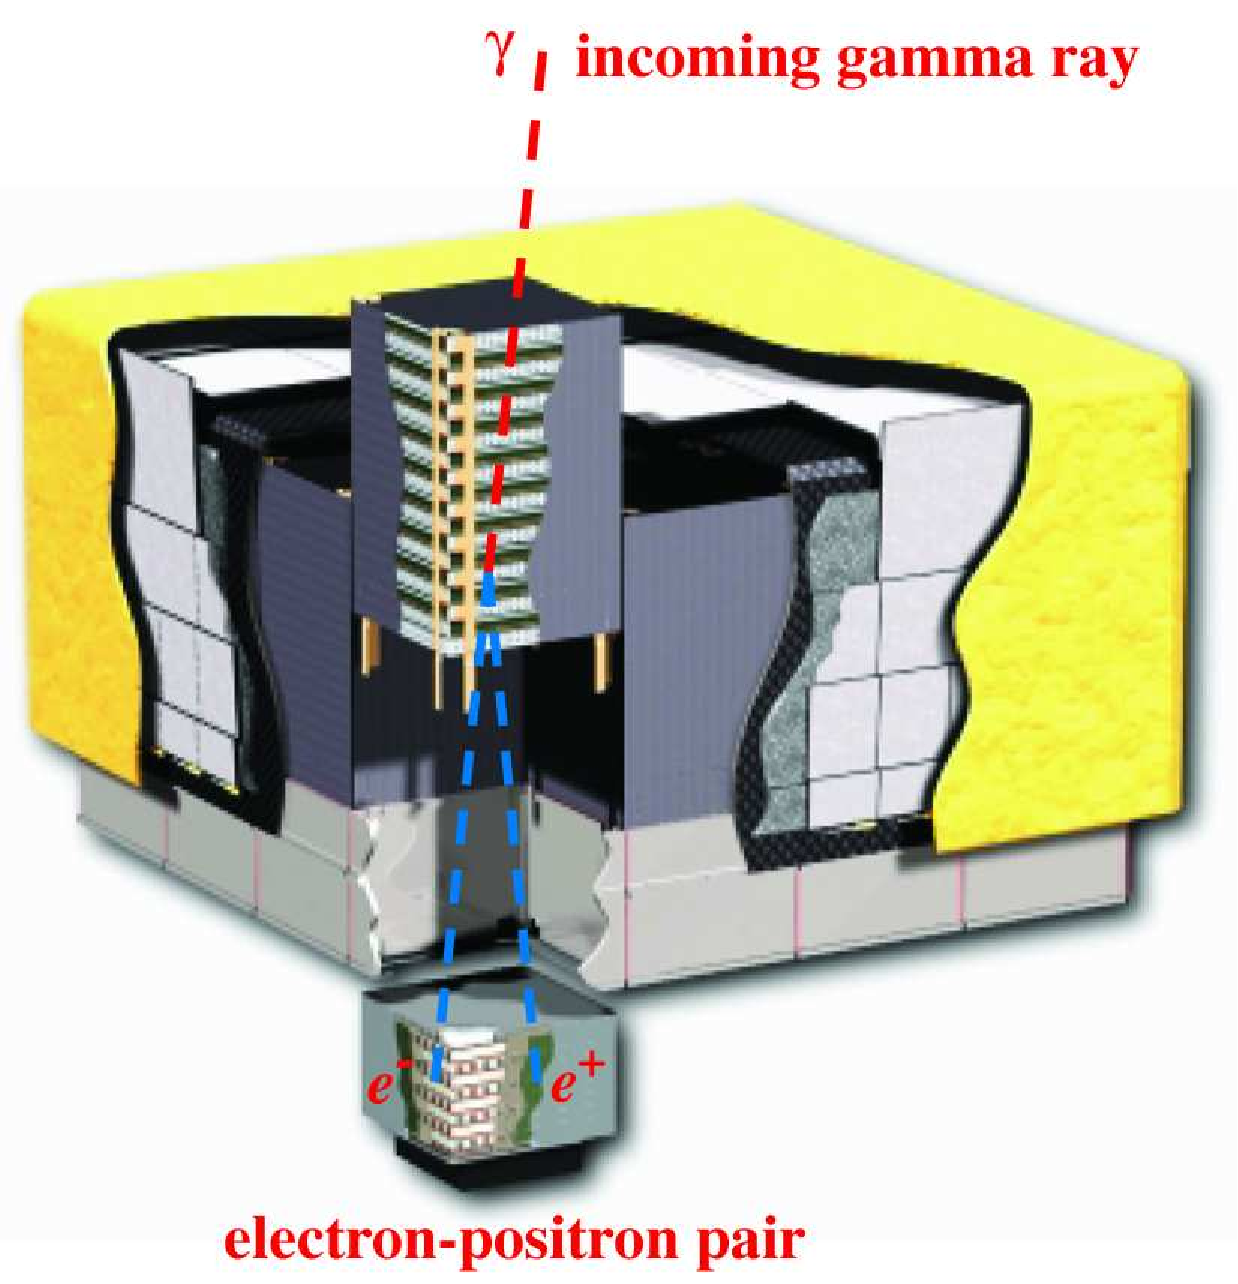
\includegraphics[width=0.60\textwidth]{Pictures/LAT.pdf}
    \caption{Schematic picture of the \gls{lat} from \cite{2009FermiLAT}. Dimensions are 1.8 m $\times$ 1.8 m $\times$ 0.72 m.}
    \label{fig:LAT}
    \end{figure}
    
    \item \textbf{The \gls{gbm}}: Complementary to the \gls{lat}, the \gls{gbm} is destined to detect \glspl{grb} and quickly alert the main instrument to reposition towards the source of interest. It is sensible to X-rays and $\gamma$-rays in the range between 8 keV to 40 MeV. The detector includes 12  \gls{nai}  scintillation detectors which cover the lower part of the spectrum (up to 1 MeV) and  provide the burst trigger, and 2 \gls{bgo} scintillation detectors with an energy range from $\sim 150$ keV to $\sim 30$ MeV, aimed to overlap the \gls{lat} energy range. 
    
    
    \begin{figure}
    \centering
    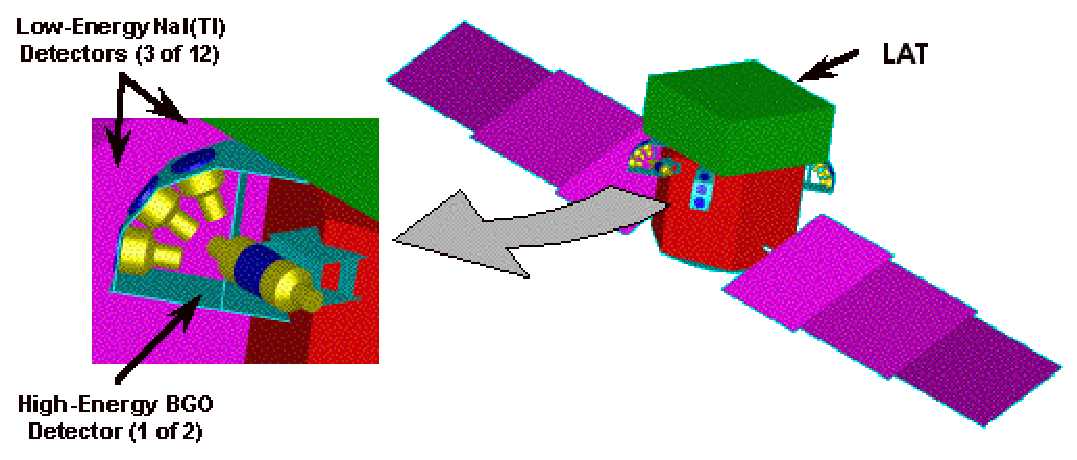
\includegraphics[width=0.75\textwidth]{Pictures/GBM.pdf}
    \caption{Schematic picture of the \gls{gbm} integrated between the \gls{lat} and the shroud envelope of the Fermi's spacecraft.}
    \label{fig:GBM}
    \end{figure}
    
\end{itemize}

The principal scientific objectives of Fermi are the study of unidentified sources detected by previous instruments like \gls{egret}; understanding the mechanisms of particle acceleration in \glspl{snr} and \glspl{grb}; studying the behaviour of \glspl{grb};performing indirect searches of Dark Matter and using $\gamma$-rays to probe the early universe and cosmic evolution of \gls{he} sources.

During the more than 10 years of data taking up to date, the \textit{Fermi}-LAT has been extremely prolific, launching several catalogs with thousands of sources. The 4FGL catalog is the last one released, based on the first 8 years of science data. It counts with 5065 detected sources above 4 sigma, 1337 of which do not have a counterpart in other wavelengths.\\
Some of the scientific highlights during its lifetime are the discovery of the mysterious Fermi Bubbles (see section \ref{sec:GCFermiBubbles}); the detection of hadronic signals in \glspl{snr} \cite{2013fermionSNRpiondecay};the detection of the most luminous \gls{grb} ever observed GRB130427A \cite{2014fermisuperGRB} and the detection with the \gls{gbm} of the \gls{grb} after the LIGO event GW170817 \cite{grb170817}, among many more. 

\section{Extensive Air Showers} \label{sec:eas}

As explained in the beginning of this chapter, the atmosphere absorbs the totality of the $\gamma$ radiation coming from space. Any $\gamma$-ray entering the atmosphere will interact with an atomic nucleus triggering the production of a cascade of particles known as \gls{eas}. Furthermore, not only $\gamma$-rays can produce \gls{eas}, but \glspl{cr} too,  being in fact the responsible for the majority of \gls{eas} happening in the atmosphere (> 99\%). The products of these cascades, whether being secondary particles or Cherenkov radiation (see section \ref{sec:cherenkov}), are the targets for ground based $\gamma$-ray detectors. Depending on the type of detector, different techniques are required to reconstruct the energy and direction of the primary particle, in addition to distinguish between electromagnetic (produced by $\gamma$-rays) and hadronic (produced by \glspl{cr}) showers. In this section, the characteristics and physical processes produced in the different types of \gls{eas} are described.

\subsection{Electromagnetic Showers}

When a primary $\gamma$-ray enters the atmosphere, it will produce a pair of $e^{\pm}$ in the electric field of an atomic nucleus, typically after traversing one radiation length ($\xi_{0}$ defined as the mean distance for a charged particle to reduce its energy by a factor \textit{e} due to interactions with the medium), at about 20 km of altitude. This pair of particles, emitted in the forward direction will again interact with other atmospheric nuclei through bremsstrahlung, producing high energy photons. The result is a chain of pair production-bremsstrahlung processes, where a certain amount of energy is lost in each interaction, until the high energy photons reach a critical energy $E_{c} \sim$ 83 MeV. When this happens, ionization and Compton scattering of electrons and positrons become dominant over bremsstrahlung so the production of high energy photons is reduced until the shower slowly dies. Since the angle of emission in all the processes is proportional to $\propto m_e c / E$ rad, the shower will not spread too much laterally, from an axis pointing towards the primary direction \cite{weekes2003HEAstrophy}. \\

 \begin{figure}
    \centering
    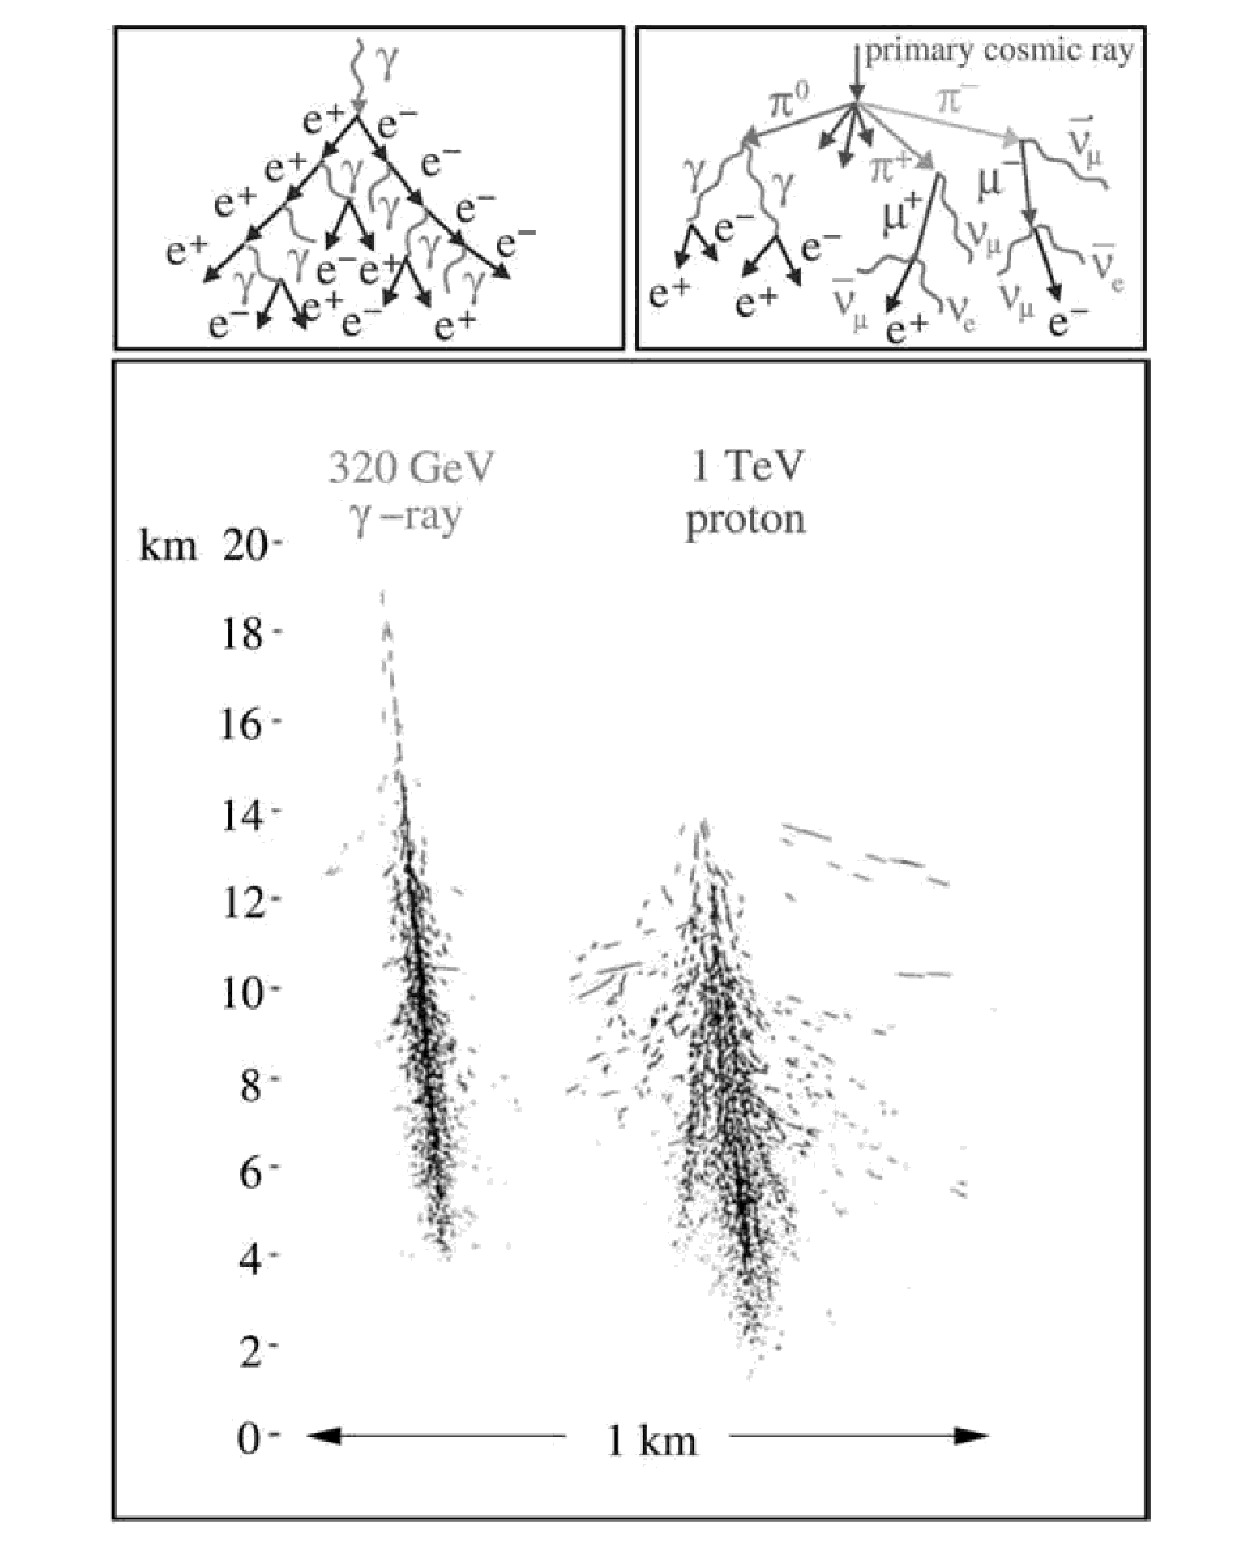
\includegraphics[width=0.75\textwidth]{Pictures/eas.pdf}
    \caption{Montecarlo simulations of a 320 GeV $\gamma$-ray shower and a 1 TeV proton shower from \cite{weekes2003HEAstrophy}. The top panel show a schematic diagram of shower development with their secondary particles.}
    \label{fig:EAS}
    \end{figure}

To understand in a simple way the evolution of the shower, It can be considered that it develops in discrete steps of one radiation length, just as in the model from \cite{1954Heitler}. The radiation length for the $e^\pm$ pair is going to be close to the mean free path of photons of similar energy ($\simeq 9/7 \xi_{0}$) which for the air is 36.7 g cm$^{-2}$. Defining the atmospheric thickness as R=$\xi_{0}ln2$, the probability of a photon, electron or positron of the shower to interact while traversing a longitude R will be exp(-R/$\xi_{0}$) = 1/2. Since the distribution of energy in each step between the charged particles and the emitted high energy photon is considered symmetric, after traversing a thickness nR, the number of surviving $e^\pm$ and photons will be $2^n$, and their mean energy $E_{\gamma}/2^{n}$, where $E_\gamma$ is the energy of the primary $\gamma$-ray. When the energy reaches the critical energy $E_c$, the shower has reached the shower maximum, where the total number of particles is $E_{\gamma}/E_c$. The position of such maximum is:

\begin{equation} \label{eq:xmax}
    X_{max} = \frac{R}{ln 2} ln \frac{E_{\gamma}}{E_c} = \xi_0 ln \frac{E_{\gamma}}{E_c}
\end{equation}

The shower maximum depends on the energy of the primary: higher energy photon showers penetrate more deeply in the atmosphere than lower energy showers, hence in order to lower the energy threshold of a ground based detector it must be located at high altitudes.\\
An analytical approach to shower development was carried out in \cite{RossiGreisenCR}. The Greisen equation defines the number of electrons, positrons and photons in the shower before reaching the critical energy:

\begin{equation}
    N_{e}(t) = 0.31 \left[log \frac{E_{\gamma}}{E_{c}}\right]^{-1/2} e^{T[1-(3/2)log\,s}
\end{equation}

Where T is defined as the atmospheric depth expressed in radiation lengths, and s is the shower age parameter:

\begin{equation}
    s = \frac{3T}{T+2ln \left[\frac{E_{\gamma}}{E_c}\right]}
\end{equation}

The age parameter s indicates the degree of development of the shower, being equal to 0  at first interaction, 1 in the shower maximum and 2 in the dying point. \\
While $N_{e}$ describes the longitudinal distribution of the shower, the lateral distribution is given by the Nishimura-Kamata-Greisen function: 

\begin{equation}
    f(r) = \frac{\Gamma(4.5-s)}{\Gamma(s)\Gamma(4.5-s)} \frac{N_e}{2\pi r^2}\left[\frac{r}{r_m} \right] \left( 1+\frac{r}{r_m} \right)^{s-4.5}
\end{equation}

Where r is the distance from the shower longitudinal axis and $r_{m}$ is the Molière radius, characteristic from multiple scattering theory,  and $\Gamma$ is the gamma function. 

\begin{figure}
    \centering
    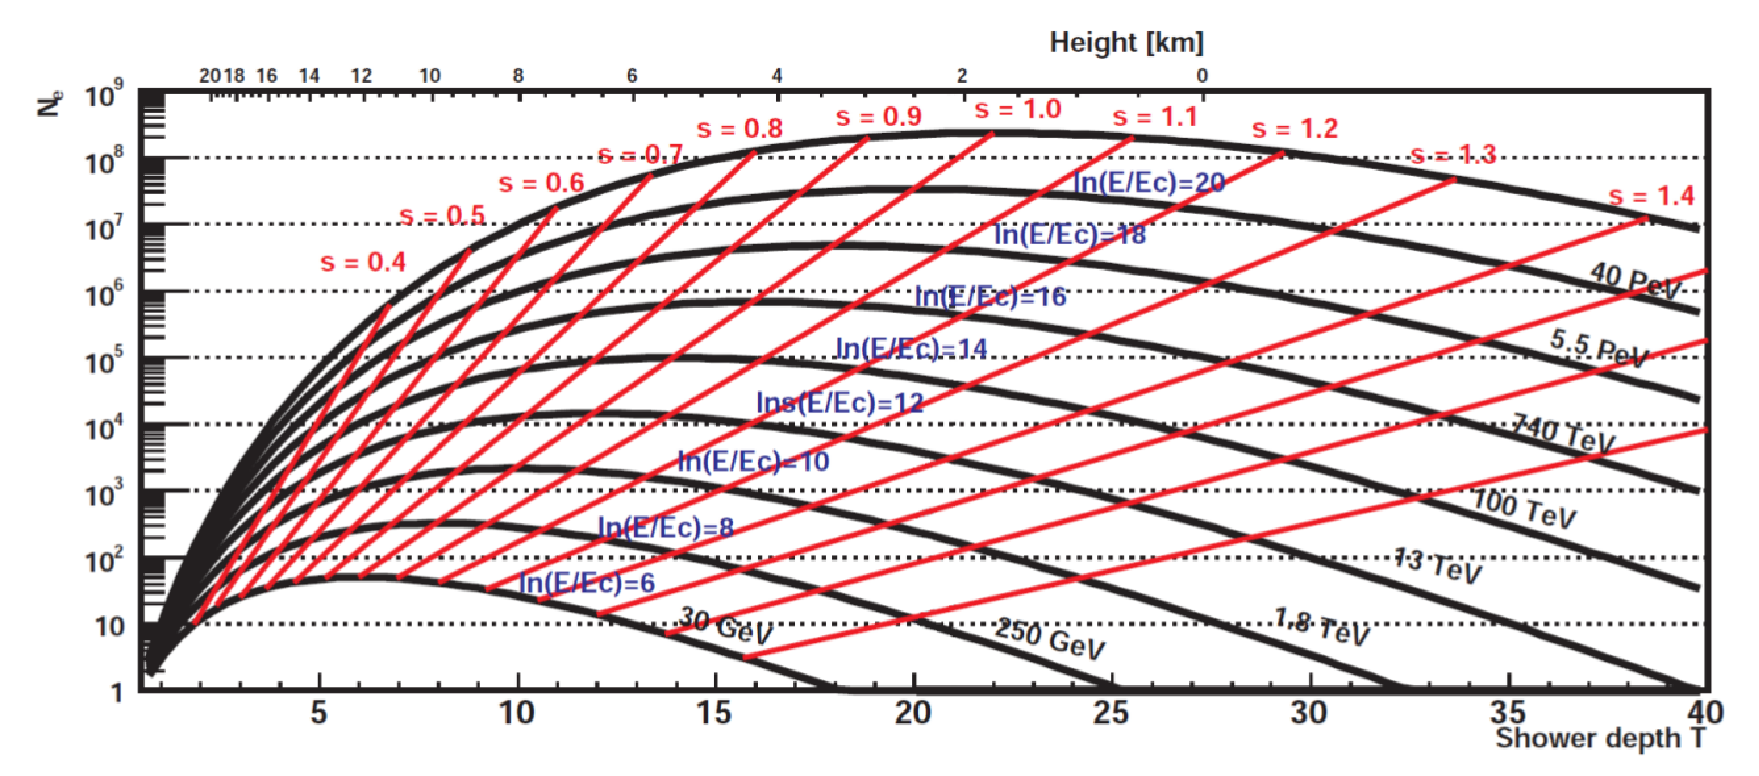
\includegraphics[width=1\textwidth]{Pictures/showerdevelop.pdf}
    \caption{Longitudinal development of an electromagnetic shower in the Greisen approximation, from \cite{IOyaThesis} and \cite{TarekThesis}.}
    \label{fig:showeredel}
\end{figure}

\subsection{Hadronic showers}

Hadronic showers are produced by \glspl{cr}, mostly protons, colliding with atmospheric particles. Their development is substantially different from electromagnetic showers, since they produce a vast number of secondary particles of different nature (see figure \ref{fig:EAS}) mainly fragments of atomic nucleus, pions and kaons, which end up decaying into muons and neutrinos. Hadronic showers have three components:\\

\begin{itemize}
    \item \textbf{Hadronic core}: In the first interaction, a relativistic \gls{cr} collides with a nucleus (O, N...) fragmenting it into smaller nucleons and transferring energy to them, which on their side keep colliding with other particles. They also produce charged mesons in each interaction ($\pi$ and K mesons). Hadronic interactions will continue until the energy per nucleon becomes smaller than the pion production threshold around 1 GeV. \\
    
    \item \textbf{Electromagnetic component}: Around 90\% of the particles generated in hadronic showers are pions, of which 1/3 are $\pi^{0}$. Neutral pions decay into two \gls{he} photons which generate pure electromagnetic showers. Charged K mesons can also decay into neutral pions through $K^\pm \longrightarrow \pi^{\pm} + \pi^0$. \\
    
    \item \textbf{Muon and neutrino component}: Charged mesons can also decay into muons and neutrinos through $\mu^{\pm} \longrightarrow \nu_{\mu}(\overline{\nu_{\mu}})$. Muons traversing the atmosphere will only lose energy through ionization due to their long life and their small bremsstrahlung cross-section. They will decay into electrons/positrons and neutrinos through $\mu^{\pm} \longrightarrow e^{\pm} + \nu_{e}(\overline{\nu_{e}})$ after a time of $2.2 \cdot 10^{-8}$ s in their own reference frame, but due to their high Lorentz factor, time dilation can make them reach ground level without decaying at all.\\ 
\end{itemize}

Despite their complexity, a model can be assumed to describe the evolution of hadronic showers, similar to the one for electromagnetic \gls{eas}. In the superposition model from \cite{2016GaisserCRandParticlePhy} it is assumed that the shower induced by a nucleus of mass A and energy $E_0$ is equivalent to A independent nuclei of energy $E_0/A$. The shower maximum in this case would be:

\begin{equation}
    X_{max} \propto \xi_{N} ln \left( \frac{E_0}{AE_c}\right)
\end{equation}

Where $E_c$ is the critical energy and $\xi_{N}$ is defined as the mean path which reduces the number of relativistic charged  particles by a factor 1/e as they pass through matter, which for a proton of 1 TeV is 83 g$cm^{-2}$. Because $\xi_{N}$ is larger than the radiation length for photons $\xi_{0}$, the altitude of first interaction of hadronic showers is higher than electromagnetic showers and they are able to penetrate deeper into the atmosphere. 
Furthermore, hadronic interactions are able to transfer considerable transverse momentum to the secondary products of the showers making them to disperse laterally. Also, hadronic showers are more irregular and present large fluctuations. These features are used in detectors to distinguish between electromagnetic and hadronic induced showers.

\subsection{Electronic showers} \label{sec:electroshowers}

There exist a third type of \gls{eas} produced by cosmic electrons and positrons entering the atmosphere. The type of cascade produced is very similar to electromagnetic showers, since the same processes take place: The electron/positron produces \gls{he} photons via bremsstrahlung while interacting in the electromagnetic field of atmospheric nuclei and those resulting photons produce $e^{\pm}$ pairs. The main differences with electromagnetic showers have to do with the nature of the primary: Since it is a charged particle, interactions start just when it enters the atmosphere so the shower maximum is reached at higher altitudes. Also, it will be more affected by the deviations produced by the geomagnetic field of the Earth.  

\section{Cherenkov radiation}\label{sec:cherenkov}

The Cherenkov radiation is a kind of electromagnetic radiation which is emitted when a charged particle travels through a dielectric medium at a velocity higher than the local speed of light. It was well observed during the \textit{XX} century when a transparent material was placed in the neighbourhood of strong radioactive sources, in the form of a faint bluish light. From 1934 to 1938 Pavel Alekseyevich Cherenkov carried out a series of exhaustive experiments to try to explain the causes of this effect and was awarded with the Nobel Prize in 1958 for his results.\\
Cherenkov radiation is a very important effect for ground-based $\gamma$-ray detectors because \gls{eas}, which contain a large number of relativistic charged particles, are able to produce this kind of radiation in the atmosphere. Characterization of the Cherenkov signal from \gls{eas} allow to trace back the nature of the primaries.\\
This effect can be explained through the reaction of the atoms of a material when a charged particle is traveling through it. For example, in the case of an electron travelling through a glass, if the electron is travelling at a slow velocity, along its trajectory the electric field of the particle will distort the atoms, attracting the positively charged nucleus and repelling the negative electrons (see figure \ref{fig:polarization} a). The medium becomes polarized around the position of the particle, each atom behaving like a dipole and the region of the glass receiving a small electromagnetic pulse. Since the distribution of dipoles  is symmetric, there will not be a resulting field thus no radiation will be emitted.

\begin{figure}
    \centering
    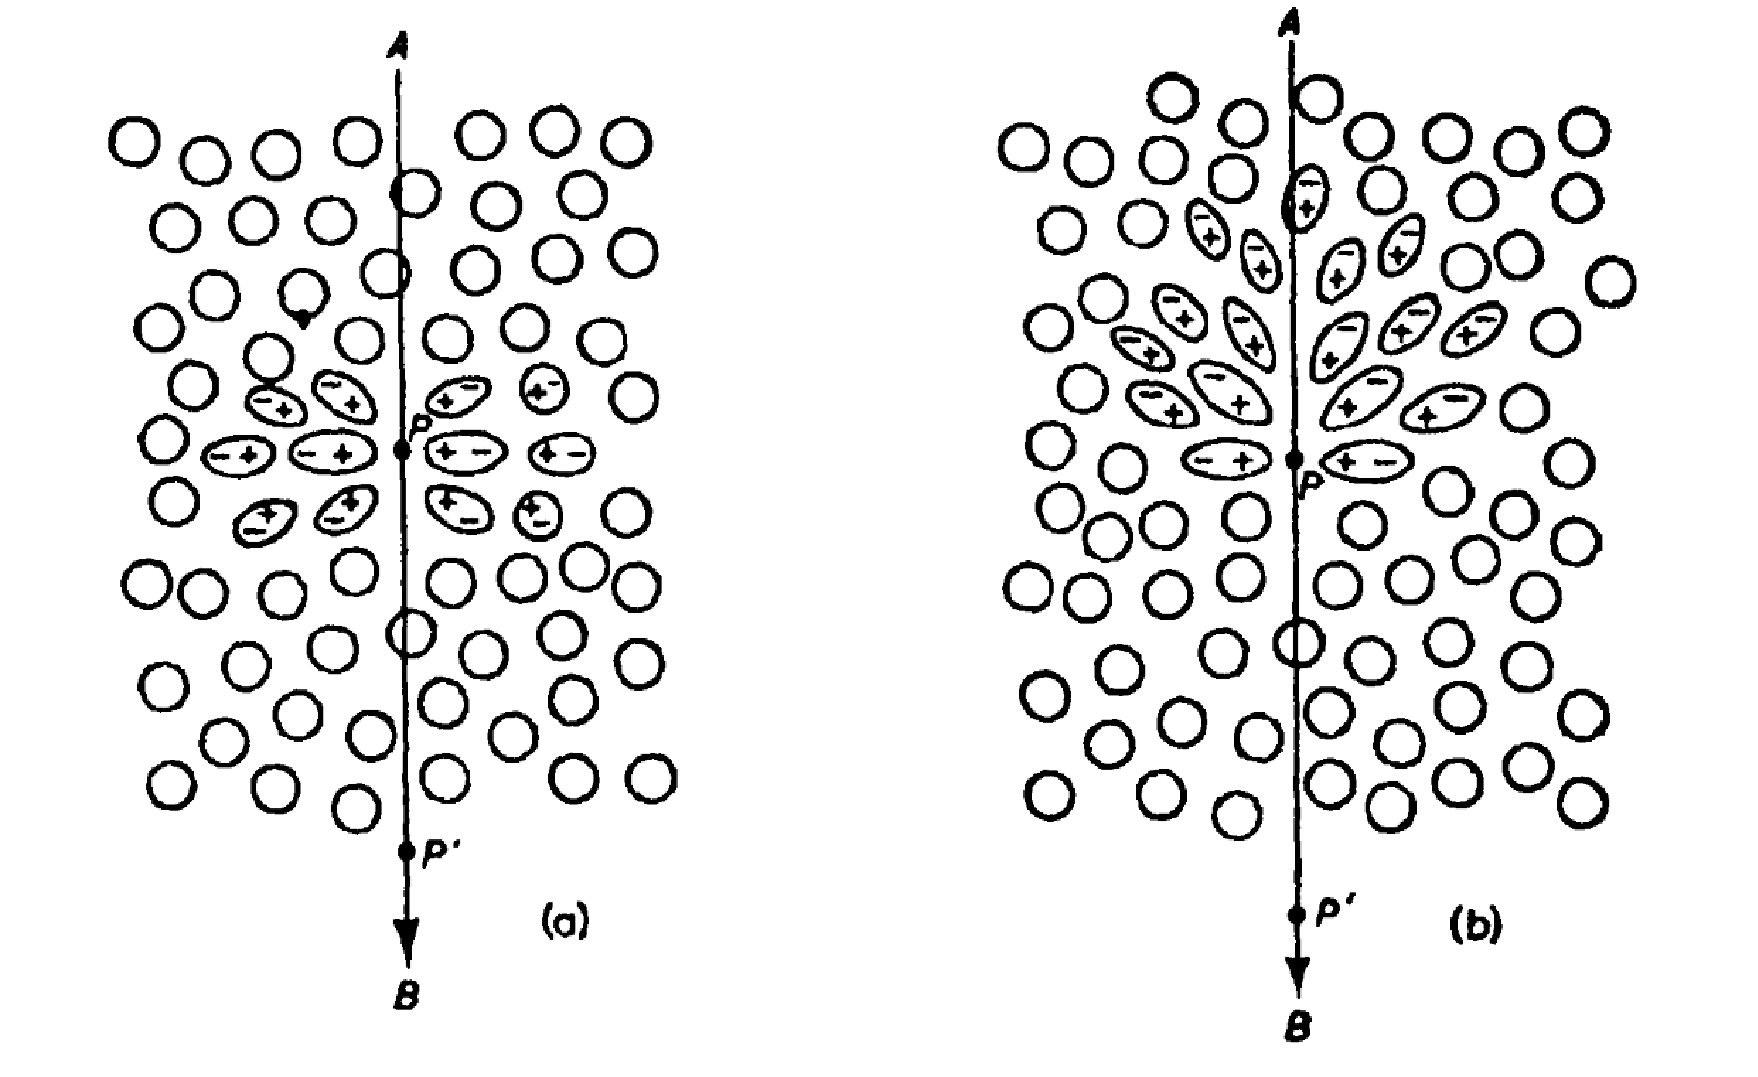
\includegraphics[width=1\textwidth]{Pictures/polarization.pdf}
    \caption{Polarization of a dielectric material at the passing of a charged particle by the point P at a) low velocity b) high velocity. Image from \cite{jelley1958Cherenkov}.}
    \label{fig:polarization}
\end{figure}

In the case the electron travels almost at the velocity of light in the medium the resulting field is not symmetric anymore along the direction axis of the particle (see \ref{fig:polarization} b). The dipole field will be noticeable even at long distances and the electron will produce the emission of wavelets of radiation at each point of its trajectory. In general, those wavelets will interfere destructively so that the resulting intensity of the field will be zero. If the velocity of the electron is higher than the speed of light in the medium, the wavelets can be in phase and produce a global field visible in the distance and thus, emit radiation. Figure \ref{fig:huygens} shows a diagram of a Huygens construction of this effect. If a particle travels from A to B faster than the speed of light in the medium, it can travel that distance in the same amount of time that light will go from A to C, therefore when seen under an angle $\theta$ all the waves emitted along the trajectory will be in phase and form a plane wave from B to C. 

\begin{figure}
    \centering
    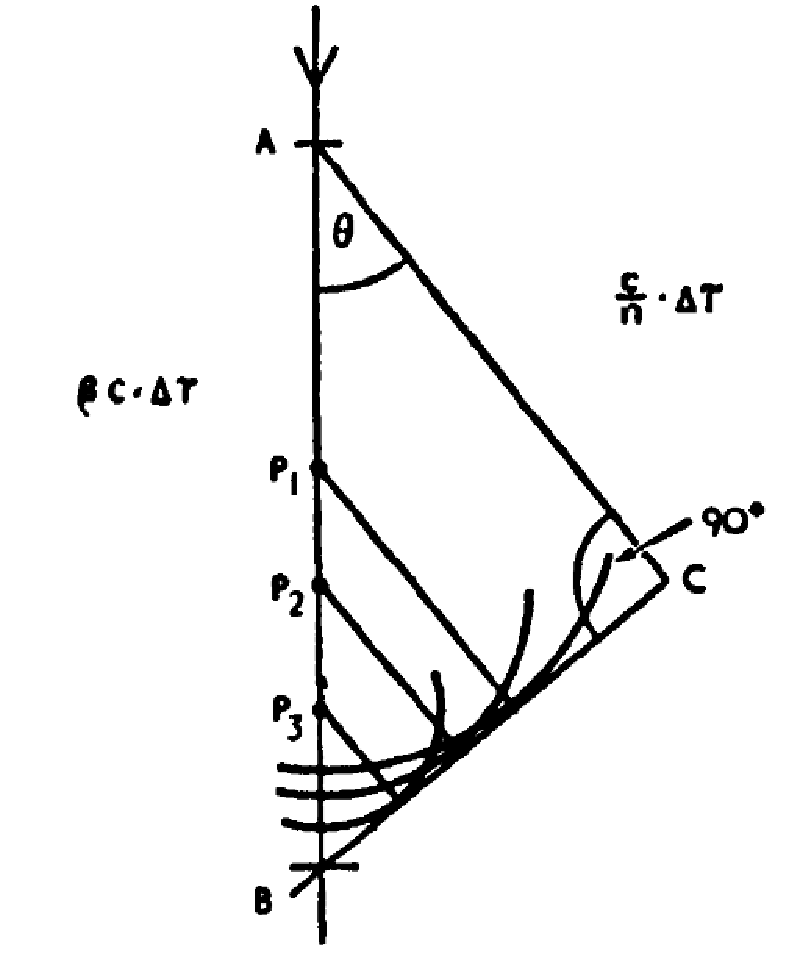
\includegraphics[width=0.6\textwidth]{Pictures/huygenscoherence.pdf}
    \caption{Diagram of Huygens construction showing coherence of waves emitted by a charged particle travelling faster than the speed of light in the medium, from \cite{jelley1958Cherenkov}.}
    \label{fig:huygens}
\end{figure}

The angle $\theta$ is named Cherenkov angle and can be expressed as:

\begin{equation}
    cos\,\theta = \frac{1}{n\beta} + \frac{\hbar k}{2p} \left( 1-\frac{1}{n^2}\right)
\end{equation}

Where $\beta = v/c$, k is the emitted photon momentum, p is the charged particle momentum and n is the refractive index of the medium. Since p $\gg$ k, the expression can be simplified to:

\begin{equation}
    cos\,\theta = \frac{1}{n\beta}
\end{equation}

The Cherenkov light produced by \gls{eas} in the atmosphere will be emitted in the shape of a cone around the axis of the shower, leaving a ringlike signal when reaching the ground. Because the refractive index of the atmosphere changes with altitude, the maximum angle will also vary and so the extension of the ring and the minimum energy required by a particle to produce Cherenkov radiation (when v = c/n).
The variation of the refractive index with altitude can be approximated by:

\begin{equation}
    n(h) = 1+n_0e^{-\frac{h}{h_0}}
\end{equation}

Where $n_{0}$ is 2.9 $\times 10^{-4}$ and $h_0 = 7.1 km$ for an isothermal atmosphere, and the minimum energy:

\begin{equation}
    E_{min} = \frac{m_ec^2}{\sqrt{1-\beta_{min}^2}} = \frac{m_ec^2}{\sqrt{1-(1/n)^2}}
\end{equation}

Hence the minimum energy as a function of altitude:

\begin{equation}
    E_{min} \approx \frac{m_0c^2}{\sqrt{2n_0}}e^{\frac{h}{2h_0}}
\end{equation}

and the maximum angle $\theta$:

\begin{equation}
    \theta_{max} = \sqrt(2n_0)e^{-\frac{h}{h_0}}
\end{equation}

This dependency means that at higher altitudes, the maximum angle is lower, so the Cherenkov signal in the ground will be less spreaded. Also, the minimum energy lowers with altitude, meaning that more developed \gls{eas} will more likely produce Cherenkov light.\\
About the spectrum of Cherenkov light in the atmosphere, while it could go from infrarred to ultraviolet, photons below 290 nm are absorbed by ozone ($O_3$), and over 800 nm by $H_2O$ and $CO_2$. Also if suffers Rayleigh dispersion and aerosol dispersion. As a result, the peak of the spectrum at a detection altitude of about 2km is around 300 nm (blue light). The Cherenkov spectrum produced by a particle with charge z and velocity $\beta$ is:

\begin{equation}
    \frac{d^2N}{dxd\lambda} = \frac{2\pi \alpha z^2}{\lambda^2}\left( 1-\frac{1}{\beta^2 n^2(\lambda)}\right)
\end{equation}

\section{Ground-based detectors} \label{sec:grounddet}

Ground-based detectors work capturing the products of \gls{eas} generated by primary $\gamma$-rays in the atmosphere. As explained in previous sections, \gls{eas} produce a cascade of particles which at the same time, emit Cherenkov light. There are two main types of ground based detectors: Particle detectors, which capture the particles produced in the shower, and Cherenkov detectors, which measure the Cherenkov light. Because both $\gamma$-rays and \glspl{cr} produce showers, the biggest challenge for ground based detectors is to differentiate the two kinds of events, being less efficient than for space detectors. A proper knowledge of the differences in the development of electromagnetic and hadronic showers is crucial for this task. In general, ground based instruments take advantage of very precise Montecarlo simulations of \gls{eas} to find features in the signals which can help to the $\gamma$/hadron separation.\\

\subsection{Particle detectors}

Particle detectors measure the particles and secondary photons produced by \gls{eas}. Because the shower maximum depends on the energy of the primary, as seen in equation \ref{eq:xmax}, only $\gamma$ rays with extremely high energies can produce showers that reach the ground. In order to lower the energy threshold of detectors is necessary to place them at high altitudes (over 2000 m). \\

\begin{itemize}
    \item \textbf{Particle counter matrices detectors} are classic particle detectors which record the arrival time of particles and direction to reconstruct the shower and eventually the primary characteristics. Examples of this kind of experiments are CASA-MIA \cite{casamia}, LHAASO-KM2 \cite{2016LHAASO}, Tibet-AS \cite{1990TibetAs} and HEGRA \cite{FONSECA1992HEGRA}.\\
    \item \textbf{Water Cherenkov detectors} are other kind of particle detector. They consist on a large number of big water tanks where particles from the shower produce Cherenkov light. ARGO-YBJ \cite{2015Argo} and HAWC \cite{2014HAWC} are examples of this kind of detector.\\

\end{itemize}
The advantage of particle detectors is that they can be extended over hundreds of square meters, covering a very wide field of view. Also, they can work anytime, even under daylight. In general they cover the higher energy range, being able to reach hundreds of TeV.

\subsection{Atmospheric Cherenkov Telescopes}

Cherenkov photons produced by \gls{eas} in the atmosphere account for $10^{-4}$\% of the \gls{nsb} and they can be observed from the ground as flashes of around 10 ns. They require very clear and dark moonless nights, unlike particle detectors. There are two types of atmospheric Cherenkov telescopes:  

\subsubsection{Sampling detectors}

They consist on a grid of counters which measure the Cherenkov light from \gls{eas} at ground level with low-gain \gls{pmt}. The direction of the primary can be determined measuring the timing signals from the photons detected, and the energy is reconstructed from the lateral distribution of the Cherenkov light. The energy threshold for these kind of detectors is high, being suitable for the study of \gls{vhe} and \gls{uhe} $\gamma$-rays. For example the minimum energy threshold of the \gls{airobicc} is 20 TeV. For sampling detectors, differentiating $\gamma$-ray showers from hadronic is truly problematic, and currently they have been outperformed by \glspl{iact}. 

\subsubsection{Imaging Atmospheric Cherenkov Telescopes}

\glspl{iact} are the most prolific type of ground based $\gamma$-ray detectors and their evolution is the key for the next generation of \gls{vhe} $\gamma$-ray astrophysics.\\
They work similar to optical telescopes, with big mirrors which collect Cherenkov light into a camera, where they record images of the showers. 
Because Cherenkov light flashes are very short, cameras need to be very fast to take snapshots of just  a few nanoseconds. Also, as \gls{nsb} is very high compared to the small number of Cherenkov photons, is essential to have a very precise time correlation between camera pixels, given by very sophisticated state-of-the art electronics, to reject random signals from \gls{nsb} and get the time evolution of the showers.\\
The reconstruction of the primary photon and the separation of $\gamma$ and hadron events can be done through a parametrization of the shower images, based on the work done by Michael Hillas \cite{1985Hillas}. With this method, moments of the light distribution in the camera, which for $\gamma$-rays look like an ellipse (named Hillas ellipse) are used as parameters to characterize the shower and allow to distinguish between $\gamma$  and hadronic showers. The quantity of Cherenkov light in the image is directly proportional to the energy of the primary and the orientation of the ellipse can be used to reconstruct their direction of arrival. Several techniques are used to reconstruct the primary information from Hillas parametrization, most of them based on modern Machine Learning algorithms.\\

\begin{figure}
    \centering
    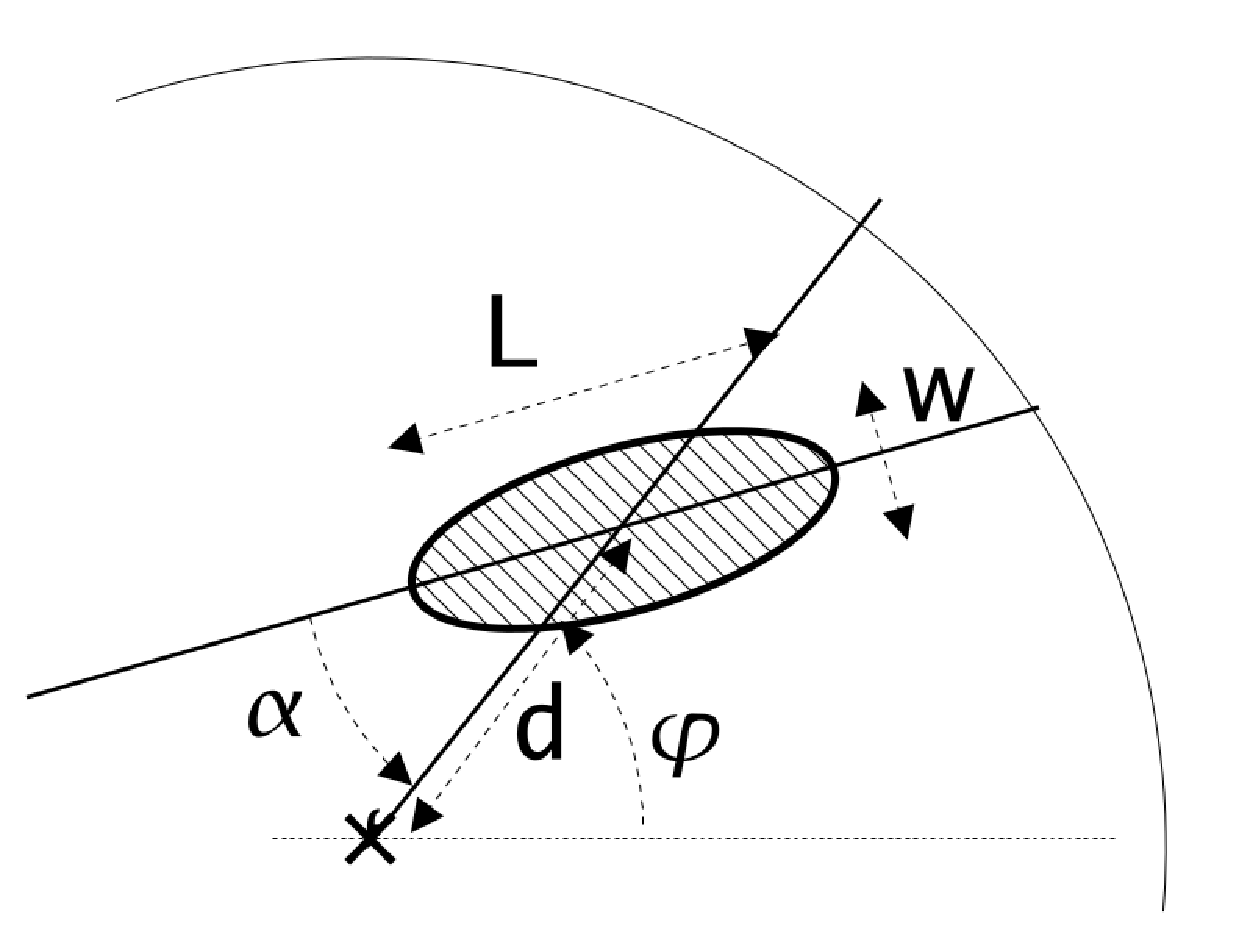
\includegraphics[width=0.6\textwidth]{Pictures/Hillaspars.pdf}
    \caption{Geometrical definition of the Hillas parameters. L for Length (W for Width) is the RMS spread of light along the major(minor) axis of the image, it carries information of the longitudinal(lateral) development of the shower. Nominal distance d is the angular distance between the centre of the camera and the image centre of gravity. Angle $\phi$ is the azimuthal angle of the image major axis and orientation angle $\alpha$ is the angle between the major axis and the center of the camera. Figure from \cite{2006analysismethodscherenkovtels}. }
    \label{fig:hillas}
\end{figure}

Other techniques further use the entire information of the camera image, comparing pixel by pixel with a template generated by a semi analytical model of shower development.\\
A detailed summary on reconstruction methods for Cherenkov Telescopes can be found in \cite{2006analysismethodscherenkovtels} and \cite{2015groundbasedtechniques}.\\

Either of the techniques improve substantially when using stereoscopy, taking shower images with several telescopes at the same time. Not only it improves the reconstruction power but also helps rejecting the hadronic background very efficiently. For example, when pointing the telescopes to a $\gamma$-ray sources, in general, shower images from $\gamma$ primaries will be oriented towards the center of the camera (the position of the source) in all telescopes. Hadronic showers, which come from random directions in the sky, will point towards random directions in the camera, so they can be easily discarded. 

\begin{figure}
    \centering
    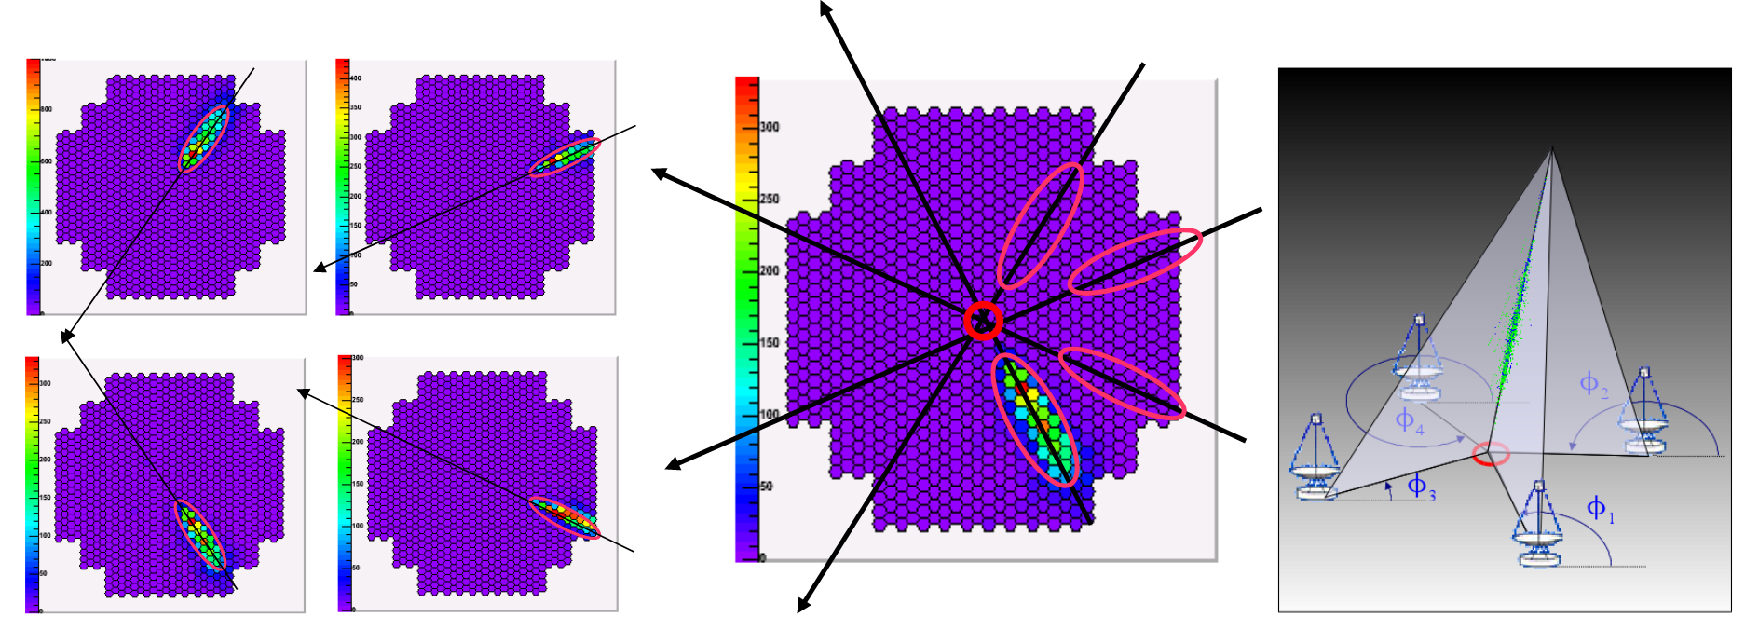
\includegraphics[width=1\textwidth]{Pictures/stereomode.pdf}
    \caption{Geometric reconstruction of shower direction in stereo mode, from \cite{2015groundbasedtechniques}. \textit{Left and middle}: The shower image from 4 telescopes is combined to get the source position in the intersection of the main axis. \textit{Right}: Intersection of the planes which contain the shower tracks and the telescopes give the shower Impact Parameter on the ground.}
    \label{fig:stereoreco}
\end{figure}

The first telescope of this kind was the Whipple Observatory 10m reflector \cite{whipple}, with a camera of 37 pixels. It started operations in 1968 but it wasn't until 1988 that they detected the first $\gamma$-ray source, the Crab Nebula. The first stereoscopic system was the \gls{hegra} complex, with a total of six \glspl{iact} which worked together with other types of $\gamma$-ray detectors (like the \gls{airobicc}).\\
The current generation of \glspl{iact} is formed by \gls{magic} \cite{2011magic}, \gls{hess} \cite{2018HESS} and \gls{veritas} \cite{2019VERITAS} telescopes:\\

\begin{itemize}
    \item \textbf{\gls{magic}:} The \gls{magic} telescopes are a set of two \glspl{iact} of 17 m diameter, located in the Roque de Los Muchachos Observatory at the Canary Island of La Palma, Spain. They are at an altitude of 2200 m, separated by 85 m. The first telescope, MAGIC-I, started operations in mono mode in 2004, and in 2009 the second telescope, MAGIC-II was included, becoming an stereoscopic system. An upgrade was made during the years 2011-2012, to reduce differences between both telescopes and improving the stereo performance.\\
    The energy threshold of \gls{magic} can reach 25 GeV when using the \textit{sum trigger} setup, becoming the most sensitive \gls{iact} system below 300 GeV in the northern hemisphere.\\
    Due to their big size, the \gls{magic} telescopes are specially well suited to observe low energy events, which produce less Cherenkov photons and require bigger mirrors. This characteristic makes them specially ideal for observing high redshift \glspl{agn} and pulsars. Also, they were designed to be very light in order to be able to do a fast repositioning to follow up \glspl{grb} alerts. The \gls{magic} collaboration announced the first detection of a \gls{grb} in January 2019 \cite{2019MAGICGRB}.\\
    During their fifteen years of operations the \gls{magic} telescopes have given prolific scientific results such as the detection in \gls{vhe} of the \gls{pwn} 3C 58, the one with the lowest luminosity and lowest flux ever detected in \gls{vhe} $\gamma$-rays; the observation of $\gamma$-ray emission from a jet originated inside the event horizon of the central \gls{bh} of the galaxy IC 310; the detection of the galaxy PKS 1441+25, one of the two most distant galaxies detected at high energies; the detection of the Crab pulsar, located inside the well known Crab \gls{pwn}; the detection of $\gamma$-rays from a gigantic explosion occurred in the galaxy QSO B0218+357 thanks to gravitational lensing; and the tracing of the source (the active blazar XS 0506+056) of a very rare cosmic neutrino event detected by IceCube experiment on September 2017 \cite{MAGICweb}. \\
    
    
    \item \textbf{\gls{hess}}: An array of 5 telescopes located in Namibia, close to the Gamsberg mountain, being the only \gls{iact} observatory in the southern hemisphere. The first four telescopes, operational since 2004, have 12 m diameter and are arranged in a square shape. The second phase of the experiment consisted in a fifth telescope of 28m of diameter, sitting in the center of the square. It was inaugurated in 2012 and contributed to lower the energy threshold. An update in the cameras of the small telescopes was performed during the years 2015-2016 improving the performance of the whole array.\\
    The energy range of \gls{hess} goes from 30 GeV to 100 TeV, being the widest of \gls{iact} observatories.\\
    Because it is located in the South, \gls{hess} has been able to perform a galactic plane survey in \gls{vhe} range, complementary to the \gls{he} survey done  by \textit{Fermi}-LAT (see picture \ref{fig:hessurvey}). Some important scientific highlights of \gls{hess} are the detection of the Vela pulsar and the colliding wind binary system Eta Carinae; the discovery of new \glspl{snr} in the galactic plane; the detection of \gls{vhe} emission from the LMC P3 binary system discovered by \textit{Fermi}-LAT, with a binary phase of $\sim$ 0.3, being the most luminous binary system detected up to date;  direct measures of the \gls{ebl} spectral density thanks to the observations of a large number of \gls{agn} spectra; and observation of flares and variability  in the \glspl{agn} Mrk 501 and 3C 279. A detailed summary on these topics among many more scientific highlights of \gls{hess} can be found in \cite{2018HESS}.\\
    
    \begin{figure}
    \centering
    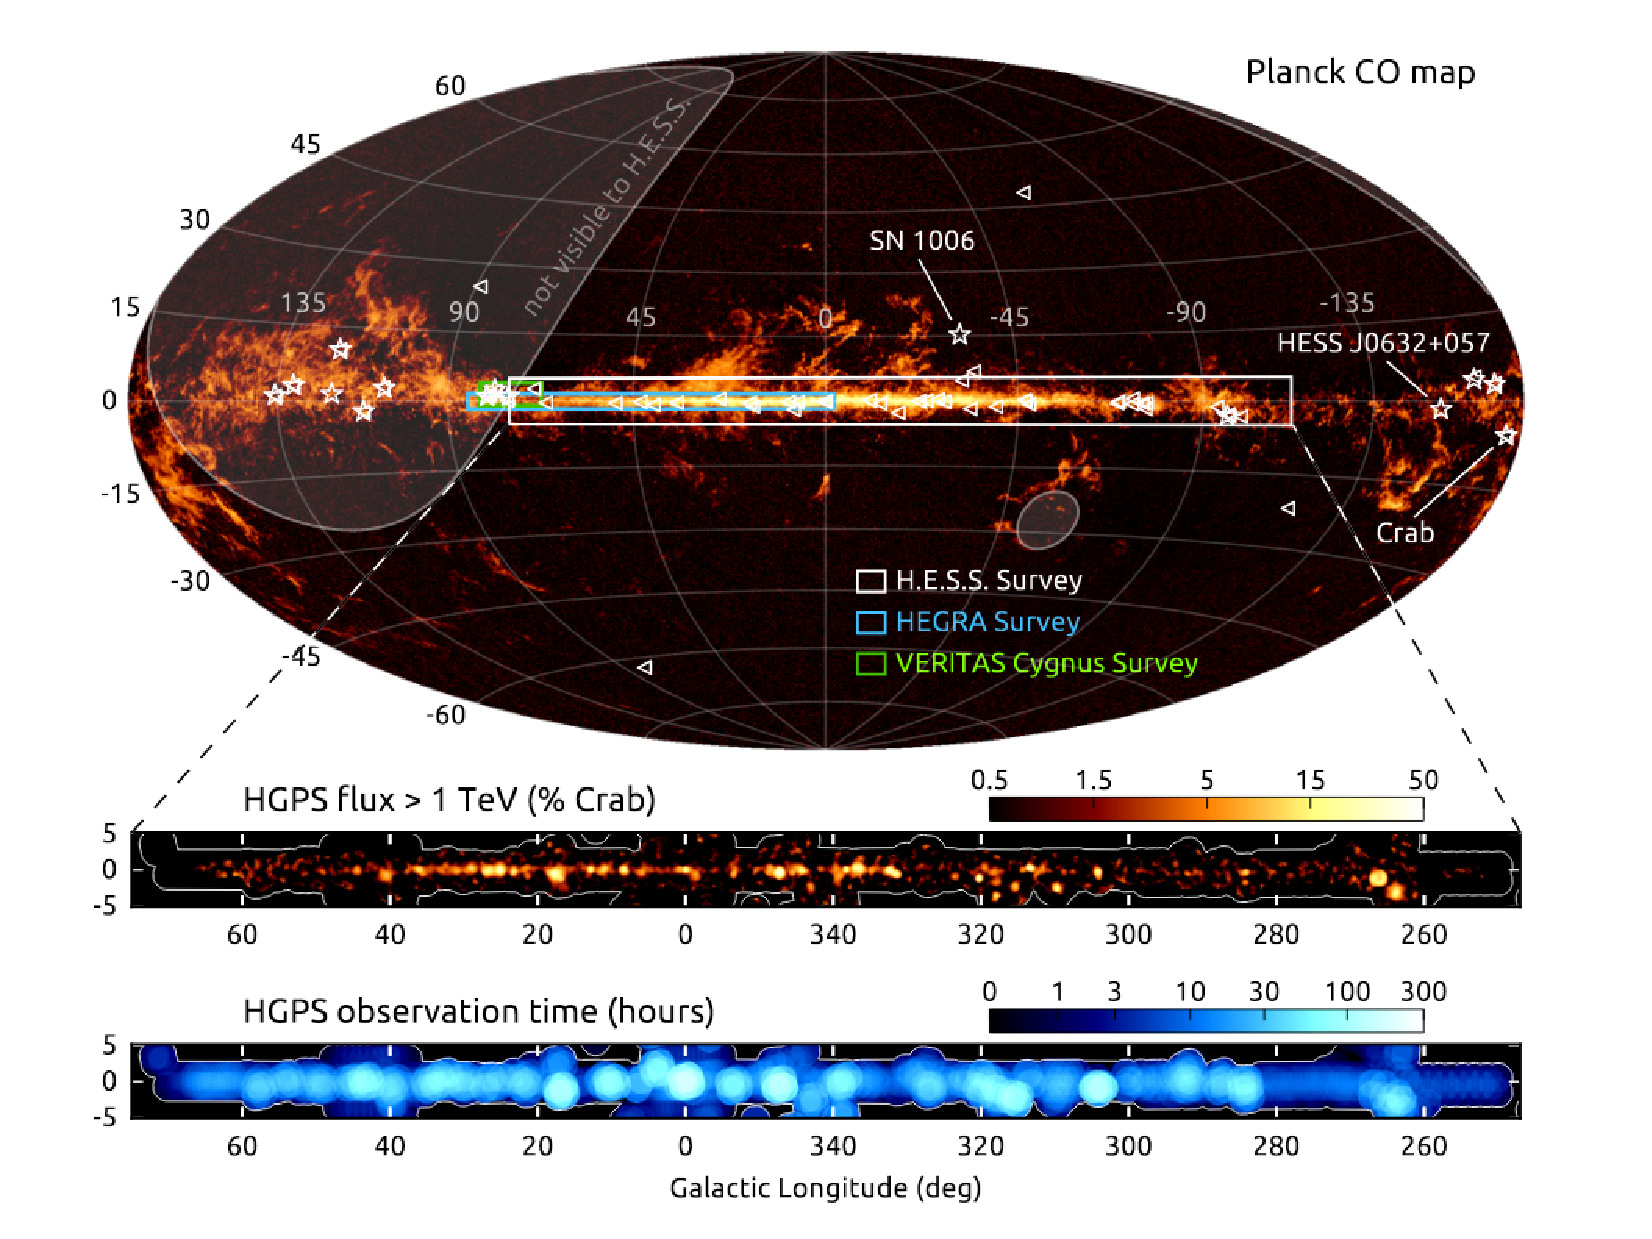
\includegraphics[width=1\textwidth]{Pictures/hesssurvey.pdf}
    \caption{Illustration of the \gls{hess} I galactic plane survey. The region surveyed is shown in the top panel as a white rectangle on top of the carbon monoxide gas sky map measured with the Planck satellite. Previous surveys from \gls{hegra} and \gls{veritas} are also represented. Triangles are sources detected at lower energies by \textit{Fermi}-LAT and stars are galactic sources detected outside the survey region. Middle and lower panels show the observed flux and observation time. Picture from \cite{2018HESS}.}
    \label{fig:hessurvey}
\end{figure}

    \item \textbf{\gls{veritas}}: Is an array of four \glspl{iact} located in the Fred Lawrence Whipple Observatory in southern Arizona. They are 12 m diameter telescopes arranged in a diamond shape and their design is based on the original Whipple 10 m Telescope. The first light of the \gls{veritas} prototype was in 2004 and the full array started operations in 2007. In 2012 the cameras \glspl{pmt} were upgraded to high-quantum-efficiency \glspl{pmt}. The total energy range goes from 85 GeV to 30 TeV. Among the most important scientific results from \gls{veritas} are the detection of pulsed emission from the Crab pulsar; Regarding the observations of blazars (\gls{agn}), the detection of rapid variability in the blazar BL Lacertae, the detection of the high redshift blazar  (z $\sim$ 0.6) PKS 1424+240 above 0.1 TeV, the discovery of the source VER J0521+211 and deep observations of the distant 1ES 0229+200 (z = 0.14); the survey of the Cygnus region which allowed to resolve new sources and contributed with new candidates of counterparts at TeV energies to \textit{Fermi}-LAT sources in the region. A summary on the most recent \gls{veritas} highlights can be found in \cite{2019VERITAS}.\\
    
\end{itemize}


The future of ground based $\gamma$-ray astronomy is in hands of the \gls{cta} currently in construction. \gls{cta} will be a $\gamma$-ray observatory without precedents, as the result of combined efforts of scientists from all over the astroparticle physics community. It will have two locations, one observatory in the northern hemisphere in the island of La Palma, Spain, and the other in the south, in the Atacama desert, Chile. This will allow to do full sky observations, with a sensitivity one order of magnitude better than the current generation of \gls{iact} observatories (see figure \ref{fig:ctaperformance}).
An extended summary on \gls{cta} can be found in chapter \ref{cap:CTA}.

\begin{figure}
    \centering
    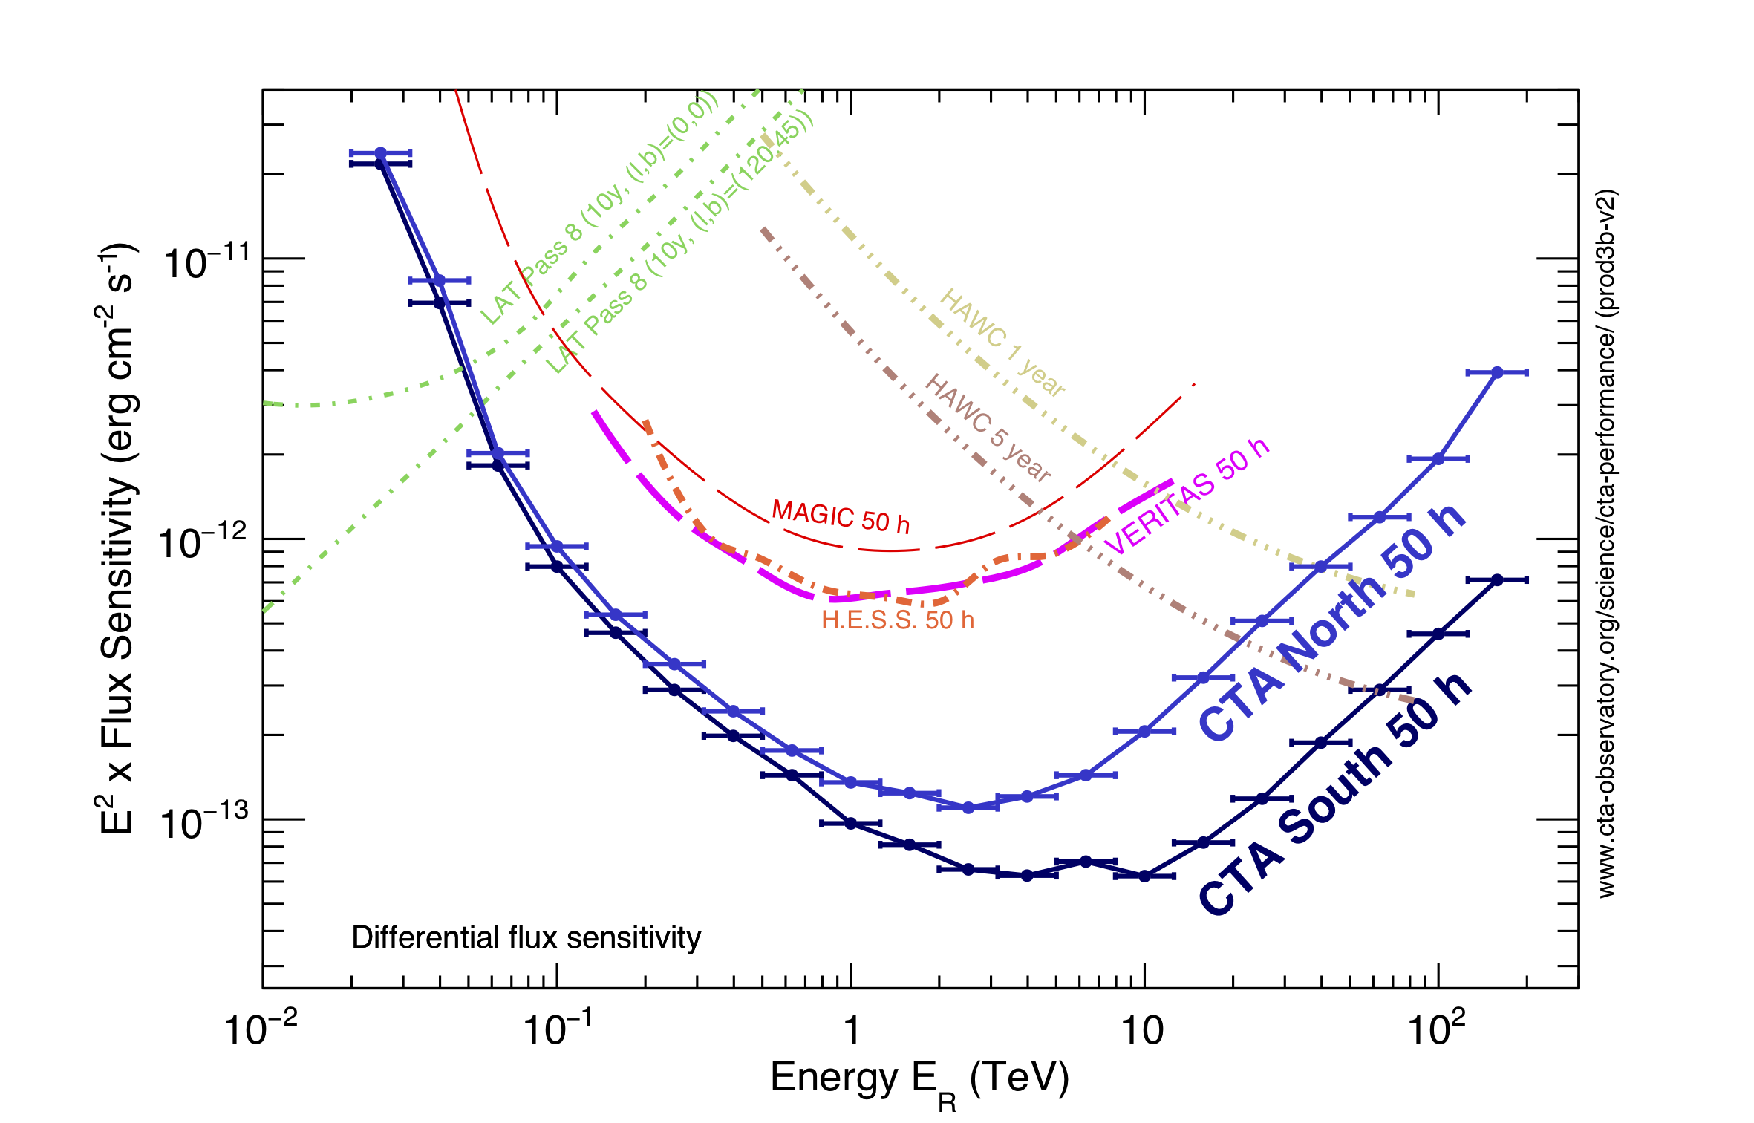
\includegraphics[width=1\textwidth]{Pictures/CTA-Performance-prod3b-v2-Comparison-DifferentialSensitivity-OtherInstruments.pdf}
    \caption{Differential sensitivity of \gls{cta} for 50 h observation compared to other $\gamma$-ray experiments, from \cite{CTAweb}.}
    \label{fig:ctaperformance}

\end{figure}



\end{document}
